%\documentclass[a4paper]{article}
\documentclass{article}
%\documentclass[journal]{IEEEtran}
%\documentclass{report}
%\documentclass{ActaOulu}

\usepackage{graphicx}
\usepackage{multirow}
\usepackage{authblk}
\usepackage{float}
\usepackage{rotating}
\usepackage{url}
\usepackage{lscape}
\usepackage{longtable}
\usepackage{subfig}
\usepackage{natbib}
\usepackage{lineno}
\usepackage{amsmath}
\usepackage{epsfig}
\usepackage{caption}
\usepackage{latexsym}
\usepackage[a4paper]{geometry}
%\setlength{\captionmargin}{20pt}
%\usepackage{graphicx}
%\usepackage[all,knot]{xy}
%\xyoption{arc}
%\usepackage{url}
%\usepackage{multimedia}
%\usepackage{hyperref}
%\linespread{1.6}
\linespread{1.2}

\newcommand{\Deg}{$^{\circ}$}
\newcommand{\Pic}[2][0.85]{\begin{center}\includegraphics[width=0.8\textwidth,height=#1\textheight,keepaspectratio]{#2}
 \end{center} }
%\newcommand{\captionfonts}{\small}
%%%%%%%%%%%%%%%%%%%%%%%%%%
% Different font in captions
\newcommand{\captionfonts}{\small}

\makeatletter  % Allow the use of @ in command names
\long\def\@makecaption#1#2{%
 \vskip\abovecaptionskip
 \sbox\@tempboxa{{\captionfonts #1: #2}}%
 \ifdim \wd\@tempboxa >\hsize
   {\captionfonts #1: #2\par}
 \else
   \hbox to\hsize{\hfil\box\@tempboxa\hfil}%
 \fi
 \vskip\belowcaptionskip}
\makeatother   % Cancel the effect of \makeatletter
%%%%%%%%%%%%%%%%%%%%%%%%%%%%
\begin{document}
\section{Numerical implementation}
Inputs to the TITAN2D code are the size and the location of the mass at 
initiation, internal and bed friction angle, and a digital elevation map (DEM)
of the topography. One of the output file produced by the code contains
the mass averaged velocity and maximum height of the pile.

As a first step of the sparse grid implementation for a hyperbolic partial 
differential system (for geophysical flows mass) high order moments of 
the output were calculated. We are going to extend 
the work of (keith),  which illustrated the MC, LHS and 
PCQ for the granular flow equations as applied to a slumping
flow of a cylinder of granular material.  
In this paper, a comparison on the convergency of the mean and standard
deviation is performed for the case when we are dealing with 2 and 4 random 
input parameters. 

% is Sparse Grid Design for the construction of a 
%hazard map. In general volcanic hazard maps are used to portray potential
%future geological events (sheridan). When a crisis develops at a volcano a 
%fast and reliable map is needed. Uncertainties in data regarding flow
%characteristics and in the construction of the DEM complicate the construction 
%of accurate hazard maps. In previous work (Stefanescu2010), a LHS design to
%sample the input space was implemented for 4 and 8 input parameters. 

Since many of the modeling applications are characterized by 
large number of input variables, TITAN2D being also the case, we try to
explore the high-dimensional input variable space and its impact on the model.
An important concern is the number of experiment or modeling simulations 
necessary to learn the effect of the system input on the output behavior.
Full space analysis without any a priori assumption has an exponential 
growing computational complexity, which leeds to some "smart" way of sampling
the parameter space. In the paper, we implemented a Sparse Grid Design (SPD) and LHS.

The following steps were performed in the analysis:
\begin{itemize}
\item Collocation points were generated in the stochastic domain
at different level of accuracy. The sparse grid toolkit \textit{spinterp}
(citation) is employed for this purpose.
\item Weights corresponding to each collocation point are determined.
\item At each collocation point, TITAN2D simulations are performed and
the relevant outputs are stored.
\item A comparison of the outputs is done for each study case.  
\end{itemize} 

\subsection{Slumping pile - 2 RV}
We considered the case of a cylindrical pile of granular material,
with a 10 cm height and radius, resting on a horizontal surface that
is suddenly released. The bed and internal friction angles have random
distributions:
\begin{equation} 
\phi_{bed} = (20 + 5\xi_1)\frac{\pi}{180} \\
\end{equation} 
\begin{equation} \nonumber
\phi_{int} = \phi_{bed} + (5 + 3\xi_2)\frac{\pi}{180}
\end{equation} 
were $\xi_1$ and $\xi_2$ are uniform distributed between -1 and 1.
We are using a Gauss-Legendre and Kronrod-Gauss-Paterson type 
sparse grid to calculate the mean and the standard deviation of averaged velocity
and maximum pile height of the pile after 3.0 seconds. In the Figure ~\ref{fig2} 
and \ref{fig3} ???it is shown the arrangements the simulations points are distributed 
in the input space. 

\subsection{Slumping pile - 4 RV}
The random variables in this study case are $\phi_{bed} \sim\mathcal{U}(15-22)$,
$\phi_{int} \sim\mathcal{U}(20-34)$, and the volume of the initial pile. The shape 
of the initial failure region is approximated as a paraboloid and gives a good
approximation of the volume range. The radius values were uniformly distributed 
between 10 and 20 mm, while the initial height followed the same distribution with values 
between 10 and 20 mm. Additional to SP runs, MC, LHS and PCQ simulations were 
performed.

\subsection{Real study case}
In the next step of our analysis we applied the computational model to
a more complex scenario. In this case are dealing with the digital terrain
representation of Mammoth Mountain, which is a large, geologically 
young volcano located on the southwestern rim of the Long Valley 
Caldera, California \citep{Bailey1989 and StefanescuM}. 
Along with uncertainties in the DEM, other four 
parameters are used to set the bounds of the computational modeling:
internal friction angle, basal friction angle, volume of the flows, and location 
of the initial pile. 
Based on the knowledge acquired from the domain expert  involved in the 
analysis and previous work in hazard analysis using TITAN2D(citation), we 
chose parameters for the flow models to bracket the range of flow volumes 
and to be representative of the friction angles that have been used by other
researchers in their computational models.  
Many TITAN2D users have chosen values of internal friction that range between
15 and 37 degrees with
values between 30 and 35 being the most frequent values used
\citep{Patra2005, murcia_2010}.  For our study we use an internal
friction angle uniformly distributed between 20 and 25 degrees.
We are using a basal friction angle
uniformly distributed between 15 and 20 degrees.
Block and ash flows on Mammoth Mountain might contain $O(10^5 -
10^7) m^3$ of material \citep{Patra2005, Burkett2007}.  Thus, our
choice of volumes ranges from $1.9 \times 10^5$ to $5 \times 10^6
m^3$.  
Initiation locations were taken from previous mapping of vent sites,
coupled with knowledge of known weak areas within the volcano as
indicated by hydrothermal alteration.  Around the centers of the
separate initiation locations, different starting positions were
uniformly distributed in a circle of radius 200 m.  

??For a better understanding of the effect of the increase in dimension
of the input space simulation for 4 RV,  and 8 RV were performed.


\begin{figure}[H]
      \begin{minipage}[b]{0.6\textwidth}
        \begin{tabular}{c}
       % \Pic[0.3]{SRTM30_dem.jpg}\\
       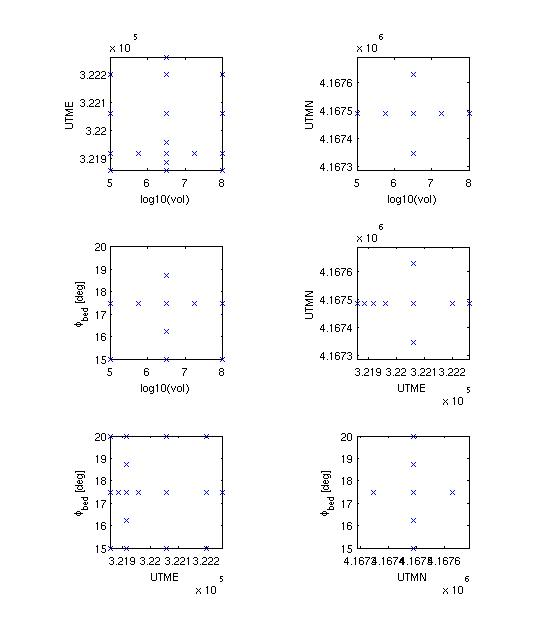
\includegraphics[width=8cm,height=9cm,keepaspectratio]{fig/picsdistrib/Clenshaw_grid.jpg}\\
        (a)
        \end{tabular}
    \end{minipage}
      \begin{minipage}[b]{0.6\textwidth}
        \begin{tabular}{c}
       % \Pic[0.3]{SRTM30_dem.jpg}\\
       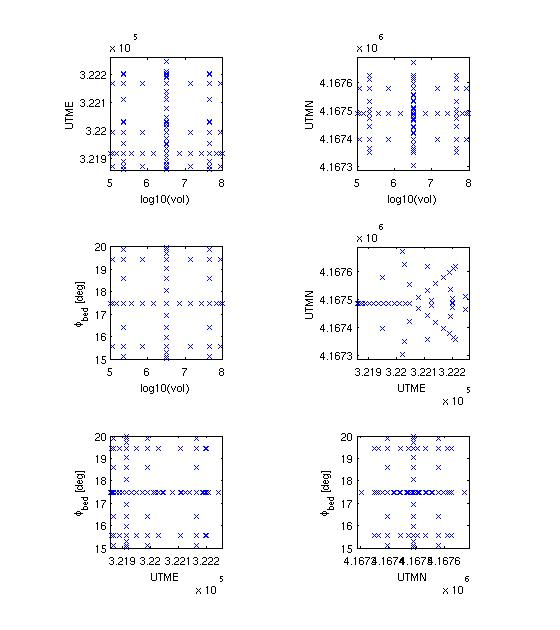
\includegraphics[width=8cm,height=9cm,keepaspectratio]{fig/picsdistrib/Clenshaw_grid_160.jpg}\\
        (b)
        \end{tabular}
    \end{minipage}
%\hfill
    \begin{minipage}{0.6\textwidth}
        \begin{tabular}{c}
       % \Pic[0.3]{NED30_dem.jpg}\\
	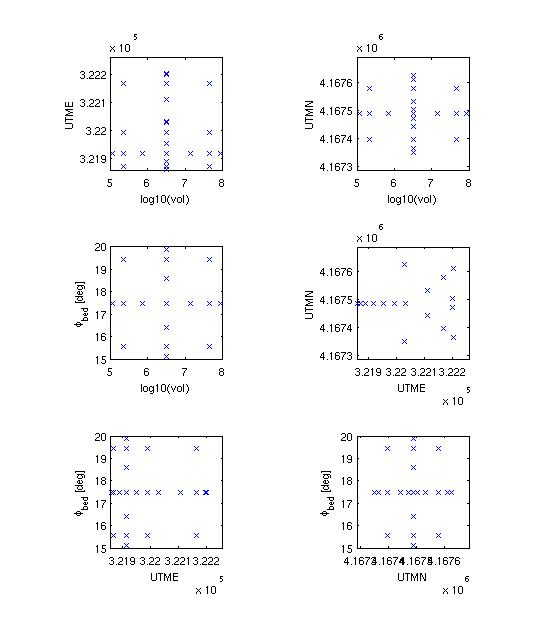
\includegraphics[width=8cm,height=9cm,keepaspectratio]{fig/picsdistrib/Gauss_Patterson.jpg}\\
        (c)
        \end{tabular}
    \end{minipage}
   % \begin{centering} 
   \begin{minipage}[c]{0.6\textwidth}
       \begin{tabular}{c}
       % \Pic[0.3]{SRTM30_dem.jpg}\\
       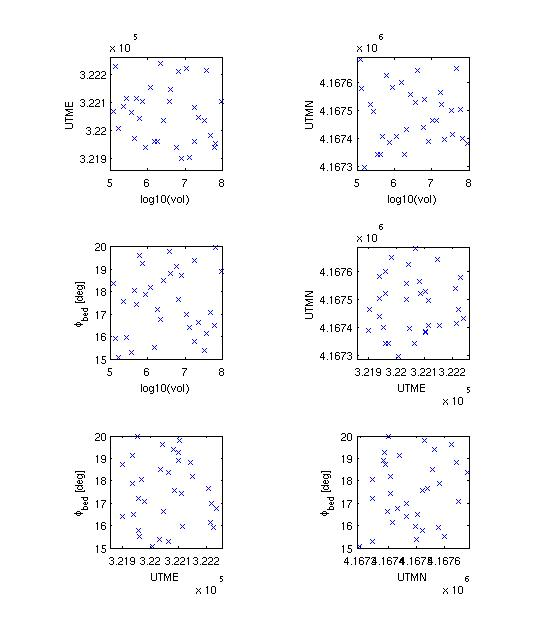
\includegraphics[width=8cm,height=9cm,keepaspectratio]{fig/picsdistrib/lhs_32.jpg}\\
        (d)
        \end{tabular}
    \end{minipage}
    %\end{centering}
\caption{ These plots are projections of a 4-dimensional random variable for a) CC - 32 sample points
b) CC - 114 sample points c) GP - 144 sample points (d) LHS -128 sample points }
\label{fig4}  
\end{figure}

\end{document}